\documentclass{report}
\usepackage[utf8]{inputenc}
\usepackage{amsmath,mathpazo,siunitx,xparse,tikz,enumitem,fancyhdr,pgfplots}

%%Needed to properly display graphs
\pgfplotsset{width=10cm,compat=1.9}

\pagestyle{fancy}
\fancyhf{}
\lhead{Steven Glasford}
\chead{Homework 2}
\rhead{Page \thepage}

\title{Homework 2}
\author{Steven Glasford}
\date{\parbox{\linewidth}{\centering%
    %%Adds the last compiled date
    \today\endgraf\medskip
    Math-451-M001}}

%%Creates a new symbol for plus and minus together
\newcommand{\rpm}{\sbox0{$1$}\sbox2{$\scriptstyle\pm$}
  \raise\dimexpr(\ht0-\ht2)/2\relax\box2 }

%%Creates a nice format for displaying the steps taken  
\newlist{steps}{enumerate}{1}
\setlist[steps, 1]{label = Step \arabic*:}

\ExplSyntaxOn
%%new command to round numbers
\newcommand*{\prlen}[1]{%
   % round to 1 digit:
    \pgfmathparse{round(10)/10.0}%
    %\pgfkeys{/pgf/number format/precision=1}
    %\pgfmathresult
    \pgfmathprintnumber[fixed, precision=2]{\pgfmathresult}
}
\ExplSyntaxOff


\begin{document}
%% adds the title to the document
\maketitle
%% adds the table of contents to the document
\tableofcontents

%%Add everything about the first problem here
\chapter{Hydro-Turbine Optimization}
\section{Introduction}
A paper company in Maine operates a hydroelectric generating station on the Penobscot River. Water is piped through from a dam to the power station. The rate at which the water flows through the pipe varies, depending on external conditions. The power station has three different hydroelectric turbine, each with a known (and unique) power function that gives the amount of electric generated as a function of the water flow arriving at the turbine. The incoming water can be apportioned in different volumes to each turbine, so the goal is to determine how to distribute water among the turbines to give the maximum total energy production for any rate of flow. Using experimental evidence and Bernoulli's equation, the following quadratic models were determined for the power output of each turbine, along with the allowable flows of operation:
\begin{align*}
    KW_1 &= (-18.89+0.1277Q_1-\num{4.08e-5}Q_1^2)(170-\num{1.6e-6}Q_T^2)\\
    KW_2 &= (-24.5+0.1358Q_2-\num{4.69e-5}Q_2^2)(170-\num{1.6e-6}Q_T^2)\\
    KW_3 &= (-27.02+0.1380Q_3-\num{3.84e-5}Q_3^2)(170-\num{1.6e-6}Q_T^2)
\end{align*}
$$250 \leq Q_1 \leq 1110, 250 \leq Q_2 \leq 1110, 250 \leq Q_3 \leq 1225$$
where

$Q_i = $ flow through turbine $i$ in cubic feet per second

$KW_i = $ power generated by turbine $i$ in kilowatts

$Q_T = $ total flow through the station in cubic feet per second


\section{Presentation of the Model}
\subsection{Objective}
\hspace{10mm} The objective of this problem is to determine the flow through each turbine needed to create the maximum amount of power.
\subsection{Variables and Constants}

\begin{center}
\begin{tabular}{c c c}
$KW_i$ &$=$ & power generated by turbine $i$ in kilowatts.\\
$Q_i$ & $=$ & flow through turbine $i$ in cubic feet per second.\\
$Q_T$ & $=$ & total flow through the station in cubic feet per second.\\
$P$ & $=$ & total power generated.

\end{tabular}
\end{center}


\subsection{Assumptions}
\begin{align*}
    KW_1 &= (-18.89+0.1277Q_1-\num{4.08e-5}Q_1^2)(170-\num{1.6e-6}Q_T^2)\\
    KW_2 &= (-24.5+0.1358Q_2-\num{4.69e-5}Q_2^2)(170-\num{1.6e-6}Q_T^2)\\
    KW_3 &= (-27.02+0.1380Q_3-\num{3.84e-5}Q_3^2)(170-\num{1.6e-6}Q_T^2)
\end{align*}
\begin{align*}
    250 &\leq Q_1 \leq 1110\\
    250 &\leq Q_2 \leq 1110\\
    250 &\leq Q_3 \leq 1225
\end{align*}
$$Q_T=Q_1+Q_2+Q_3$$
$$P = KW_1+KW_2+KW_3$$

\section{Solving the Model}
We will be using Lagrange Multipliers to find the values for the individual flow (as functions of $Q_T$) that maximize the total energy production $KW_1+KW_2+KW_3$ subject to the constraints $Q_1+Q_2+Q_3=Q_T$ and the domain restrictions on each $Q_i$.

But first we must find the objective function, which is the function we are trying to optimize. In this case it is the function $P$.
$$P = KW_1+KW_2+KW_3$$
Then we must populate this function using the data we are concerned about, we are not concerned with the optimum power generated with respect to the total power outputs of each individual turbine, instead we want to optimize with respect to the flow rates to each individual turbine. This makes the power function look more like this

\begin{multiline}
$P = (-18.89+0.1277Q_1-\num{4.08e-5}Q_1^2)(170-\num{1.6e-6}Q_T^2) + (-24.5+0.1358Q_2-\num{4.69e-5}Q_2^2)(170-\num{1.6e-6}Q_T^2) + (-27.02+0.1380Q_3-\num{3.84e-5}Q_3^2)(170-\num{1.6e-6}Q_T^2)$
\end{multiline}

Lagrange Multipliers have the form:
$$\nabla f = \lambda \nabla g,$$

where $f$ is our objective function and $g$ is the constraint equation. In this problem our constraint equation is $$Q_T = Q_1 + Q_2 + Q_3$$ and $$f = P,$$ but before we continue we must replace the all of the $Q_T$ in the objective equation with the variable $Q_1, Q_2, Q_3$ which isn't difficult since the constraint equation already does this step for us.

\vspace{5mm}

\begin{tabular}{c c}
$P =& (-18.89+0.1277Q_1-\num{4.08e-5}Q_1^2)(170-\num{1.6e-6}* \\ 
&(Q_T)^2)+ (-24.5+0.1358Q_2-\num{4.69e-5}Q_2^2)* \\ 
&(170-\num{1.6e-6}(Q_T)^2) \\
&+ (-27.02+0.1380Q_3-\num{3.84e-5}Q_3^2)*\\
&(170-\num{1.6e-6}(Q_T)^2)$
\end{tabular}

%(170-w^2/625000)*(-(51*x^2)/1250000+(1277*x)/10000-1889/100)+(170-w^2/625000)*(-(3*z^2)/78125+(69*z)/500-1351/50)+(170-w^2/625000)*(-(469*y^2)/10000000+(679*y)/5000-49/2)

\vspace{5mm}

We shall try to find the extrema for P the old fashion way, by simply finding the gradient of P, then setting the gradient to 0 and finding min and maxes. To make our lives easier we will assume that $Q_T$ is a constant, which will end up making life much, much easier in the long run.
$$\nabla P = \left\langle\frac{\partial P}{\partial Q_1},\frac{\partial P}{\partial Q_2},\frac{\partial P}{\partial Q_3}\right\rangle$$

Now we must find the partials:

$$\frac{\partial P}{\partial Q_1} = \dfrac{\left(Q_T^2-106250000\right)\left(102Q_1-159625\right)}{781250000000}$$

$$\frac{\partial P}{\partial Q_2}=\dfrac{7\left(Q_T^2-106250000\right)\left(67Q_2-97000\right)}{3125000000000}$$

$$\frac{\partial P}{\partial Q_3} = \dfrac{3\left(Q_T^2-106250000\right)\left(8Q_3-14375\right)}{195312500000}$$

\vspace{5mm}

The roots of P:
$$\nabla P = \left\langle \dfrac{159625}{102},\dfrac{97000}{67},\dfrac{14375}{8}\right\rangle$$
Or more approximately:
$$\nabla P \approx \left\langle1564.95098,1447.76119,1796.875\right\rangle$$

However, this extrema is outside our bounds for all of the variables so we cannot use this method of finding the gradient and the roots of the gradient. So we must now use Lagrange multipliers. 



\vspace{5mm}
Lagrange multipliers are in the form $$\nabla f = \lambda \nabla g,$$ where $f$ is our objective equation ($P$) and $g$ ($Q_T$) is out constraint equation and $\lambda$ is our Lagrange multiplier. 

We have already found $\nabla P$ so we must now find the gradient of $Q_T$ The gradient of $Q_T$ 
$$\nabla Q_T = \left\langle\frac{\partial Q_T}{\partial Q_1},\frac{\partial Q_T}{\partial Q_2},\frac{\partial Q_T}{\partial Q_3}\right\rangle$$ which boils down to $$\nabla Q_T = \left\langle1,1,1\right\rangle$$

Now we can set the two equations equal to each other:

$$\frac{\partial P}{\partial Q_1} = \dfrac{\left(Q_T^2-106250000\right)\left(102Q_1-159625\right)}{781250000000}=\lambda$$
$$\frac{\partial P}{\partial Q_2}=\dfrac{7\left(Q_T^2-106250000\right)\left(67Q_2-97000\right)}{3125000000000}=\lambda$$
$$\frac{\partial P}{\partial Q_3} = \dfrac{3\left(Q_T^2-106250000\right)\left(8Q_3-14375\right)}{195312500000} = \lambda$$

and $$Q_T=Q_1+Q_2+Q_3$$

Now we want to solve for $\lambda$

$$Q_1 = \frac{15925Q_T+781250000000\lambda -1692031250000}{102Q_T-10837500000}$$
$$Q_2 = \frac{679000Q_T + 3125000000000\lambda - 72143750000000}{469Q_T^2-49831250000}$$
$$Q_3 = \frac{43125Q_t^2+195312500000\lambda - 4582031250000}{24Q_T^2-2550000000}$$

Put these equations into the original $Q_T$ equation and solve for $\lambda$

$$\lambda = \frac{7\left(2733Q_T-92963275\right)\left(Q_T^2-106250000\right)}{4297851562500000}$$

Plugging $\lambda$ back into the original $Q_i$ equations and then simplifying we get:

$$Q_1 = \frac{7501Q_T}{22005}-\frac{26500495}{26406}$$

$$Q_2=\frac{2176Q_T}{7335}+\frac{1931560}{4401}$$

$$Q_3=\frac{7973Q_T}{22005}+\frac{14911135}{26406}$$

Now we graph the function between the bounds of each variable and try to find some intersection points between the $Q_i$ functions:

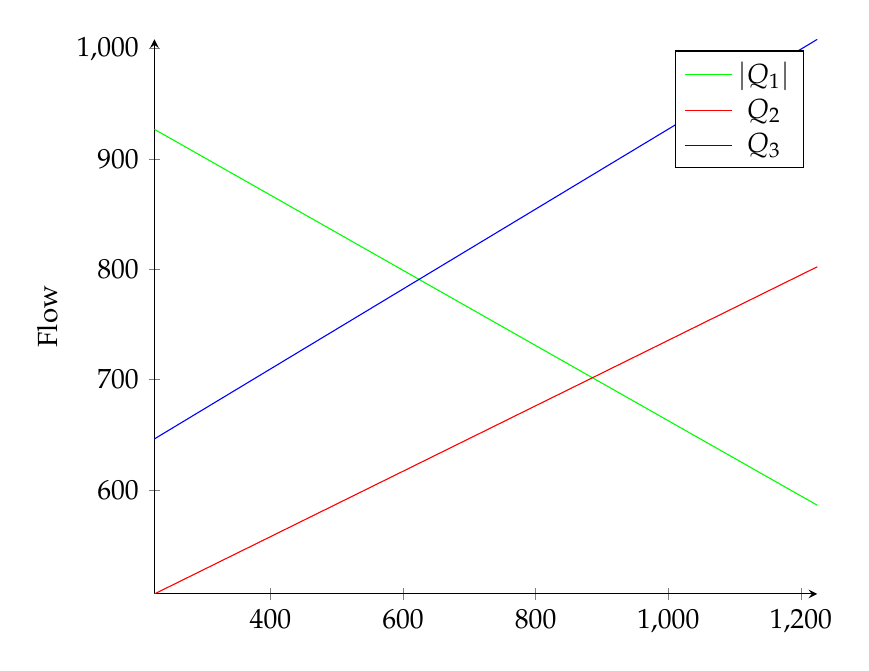
\begin{tikzpicture}
        \begin{axis}[
            axis lines = left,
            ylabel = Flow,
        ]
        
        \addplot[
            domain=225:1225,
            samples=100,
            color=green,
        ]{abs(-.3408770734*x+1003.57854276)};
        \addlegendentry{$\left|Q_1\right|$}
        \addplot [
            domain=225:1225,
            samples=100,
            color=red,
        ]{(.29665985003)*x+438.8911611};
        \addlegendentry{$Q_2$}
        
        \addplot[
            domain=225:1225,
            samples=100,
            color=blue,
        ]{(.36232674392)*x+564.687381656};
        \addlegendentry{$Q_3$}
        
        \end{axis}
    \end{tikzpicture}
    
 %   Then the optimized version of this model should be at $$790.827$$ $$Q_2=701.653$$ $$Q_3=746.24$$ for a total power generation of 16622.69864 Kilowatts.
    
  %  But then I started to think about it. Logically if you have a turbine, that turbine should generate the most amount of power when it is doing the most amount of work, which would logically place the max value at the max boundary for each individual turbine, which means the max values should be at $$Q_1=1110$$ $$Q_1=1110$$ $$Q_3=1225$$ and if you put those values into the calculator you get an even higher value than you would get from the the other values. In particular you get a total power generation of 23155.92823 kilowatts, which is obviously greater than 16622.69864, so this is a bigger maximum, and a very obvious maximum.

%$$Q_1 = -z-y \pm %2500\cdot\sqrt{17}$$

%and
%$$Q_1 = \dfrac{\sqrt{2}\sqrt{-19584Q_3^2+70380000Q_3-23919Q_2^2+69258000Q_2+15051181250} \pm 319250}{204}$$

%$$Q_2 = -Q_3-Q_1 \pm 2500\cdot\sqrt{17}$$
%and 
%$$Q_2 = \dfrac{2\cdot\sqrt{14}\sqrt{-3216Q_3^2+11557500Q_3-3417Q_1^2+10694875Q_1+2336037500} \pm 679000}{469}$$

%$$Q_3 = -Q_2-Q_1 \pm 2500\cdot\sqrt{17}$$
%and
%$$Q_3 = \dfrac{\sqrt{6}\sqrt{-469Q_2^2+1358000Q_2-408Q_1^2+1277000Q_1+535743750}\pm 86250}{48}$$

%As you may have noticed, each axis has a root something with $\pm 2500\cdot\sqrt{17}$, these would be nice to use if they pass all of the constraints of the problem, however, they fail $Q_T=Q_1+Q_2+Q_3$ since you can rearrange any of those equations to be in the form $$\pm 2500\cdot\sqrt{17} = Q_1 + Q_2 + Q_3$$ So these equations cannot be used if you consider that $750 \leq Q_T \leq 3445$, which are the combined bounds of $Q_1,Q_2,Q_3$ and $\pm 2500\cdot\sqrt{17}$ is far from being in that bound.

%%$$P = (-18.89+0.1277Q_1-\num{4.08e-5}Q_1^2)(170-\num{1.6e-6}Q_T^2) + (-24.5+0.1358Q_2-\num{4.69e-5}Q_2^2)(170-\num{1.6e-6}Q_T^2) + (-27.02+0.1380Q_3-\num{3.84e-5}Q_3^2)(170-\num{1.6e-6}Q_T^2)$$

%%$$P = (-18.89+0.1277x-4.08*10^-5*x^2)(170-1.6*10^-6*(x+y+z)^2) + (-24.5+0.1358y-4.69*10^-5*y^2)(170-1.6*10^-6*(x+y+z)^2) + (-27.02+0.1380z-3.84*10^-5*z^2)(170-1.6*10^-6*(x+y+z)^2)$$

%\section{Discussion of Results}
%\subsection{Verification}
%To verify that this is in fact the optimal flow rate to each turbine we will try some nearby distributions.

%If we try the points (1110,1110,1224), (1109,1110,1225), (1110,1109,1225), (1109,1109,1224) which are all points a little less than the max we get the following distributions

%\begin{center}
%\begin{tabular}{c c}
%     $P(1110,1110,1224)=$& 23150.97440\\
%%     $P(1109,1110,1225)=$& 23157.57594\\
%     $P(1110,1109,1225)=$& 23152.82133\\
%     $P(1109,1109,1224)=$& 23149.51208
%\end{tabular}
%\end{center}

%all of these points are less than the max, making the (1110,1110,1225) a max

\section{More Information}

\subsection{Turbine Distribution for a Predetermined Max Flow Rate}
If the incoming flow never goes beyond 2500 cubic feet per second, the flow must be distributed accordingly to maximize the power generated. As shown in the graph, $Q_2$ maxes at 701.653 and $Q_3$ at 74.24, we then allow the remaining water to flow through $Q_1$ this will result in the max for the situation.


\subsection{More Information}

\hspace{10mm} \emph{Turbines to be used if only two are allowed to operate}


If we were to have 1500 cubic feet per second, I would recommend using the $Q_2$ and $Q_3$ due to these ones generating the most amount of power individually.

\subsection{Recomendation of When the Flow Rate is Near the Hypothetical Maximum Flow Rate of Each Turbine}

If there was an incoming flow rate of 3400 cubic feet per second I would recommend allowing the maximum allowed flow through both $Q_2$ and $Q_3$, and then allowing the rest of the water to go through $Q_1$, this would generate the greatest amount of power for the situation.

\section{Conclusion}
Overall, the best point for the water distribution is when $Q_1 \approx 790.827$, $Q_2 \approx 701.53$ and $Q_3 = 24.24$ for $\approx$ of 16622.984 kilowatts.


\vspace{5mm}

\hspace{5mm} Let's say that the company discovers that it is sometimes advantageous to only use two turbines, and the incoming flow is 1500 cubic feet per second, the company should use the turbine x and turbine y to generate the most power
\vspace{5mm}

\hspace{5mm} If the incoming flow is 3400 cubic feet per second, the company should take the following action.


%%Add everything about the second problem here
\chapter{Advertising Budget Analysis for a Personal Computer Manufacturer}
\section{Introduction}
\emph{This is a problem can be found on page 52 number 6 of \textit{Mathematical Modeling, Fourth Edition} by Mark M. Meerschaert.}

\vspace{5mm}
A manufacturer of personal computers currently sells 10,000 units per month of a basic model. The cost of manufacture is \$700/unit, and the wholesale price is \$950. During the last quarter the manufacturer lowered the price \$100 in a few test markets, and the result was a 50\% increase in sales. The company has been advertising its product nationwide at a cost of \$50,000 per month. The advertising agency claims that increasing the advertising budget by \$10,000/month would result in a sales increase of 200 units/month. Management has agreed to consider an increase in the advertising budget to no more than \$100,000/month.

\section{Presentation of the Model}
\subsection{Objective}
Will try to find a price and the advertising budget size that will maximize the total revenue for this manufacturing company.

\subsection{Variables and Constants}
\begin{tabular}{c c}
    $R= $ & revenue (\$)\\
    $P= $ & profit (\$)\\
    $C= $ & costs (\$)\\
    $U= $ & units of personal computers\\
    $B= $ & advertising budget (\$/month)\\
    $S= $ & selling wholesale price per unit\\
    $D = $& price drop\\
    $B_i = $& budget increase\\
    $C_m=700=$ & cost to manufacture per unit (in dollars)  \\
    $B_0=50000=$ & initial advertising budget size\\
    $B_m=100000=$ & max advertising budget\\
    $U_0 = 10000=$ & initial number of units sold\\
    $S_0 = 950=$ &initial wholesale price
\end{tabular}

\subsection{Assumptions}
\begin{center}
\begin{tabular}{c}
    $P=R-C$   \\
    $p=S_0-D$\\
    $R = UP$\\
    $C= B + C_m*U$\\
    $B = B_0 + B_i$\\
    $U=U_0+(950-S)*50 + \frac{b-B_0}{U_0}*200$\\
    $B_0 \leq B \leq B_m$\\
    $700\leq P \leq 950$
    
\end{tabular}
\end{center}

\emph{objective:} Maximize Profits

%Notice how the equation for $U$ has two main components, the next component is the increase of sets sold as the budget for advertising increases which is a linear component since for every dollar increase the number of sets grows at a known amount, in this case by 200. Then there is a quadratic function with very interesting, seemingly random coefficients. This part of the equation was found using a calculator doing linear regressions on the points:
%\begin{center}
%\begin{tabular}{c}
 %   (950,10000)\\
  %  (850,15000)\\
   % (750,22500)
%\end{tabular}
%\end{center}

%I chose those points due to the 50\% increase of sets purchased as a \$100 decrease in price. I then put these points into the calculator to find a regression between all of them. I could have chosen to use a more exact regression and more points (this would also reduce the overall amount of error in the model, however I felt that this regressed version might be easier to have a calculator use later on in the problem. I chose to do a quadratic regression because the correlation between the points and the function is 1. I could have used a cubic or quadratic regression with added points, however I felt that those would have added too much complexity.

\section{Solution to Model}
In order to proceed we need to obtain our objective function

%We will model this as a constrained optimization problem, and solve it using the method of Lagrange multipliers.

%First we must make a uniform objective equation, which uses the variables $B$ and $S$:

$$P=R-C$$

$$\left(10000+(950-p)50+\frac{B-50000}{10000}\cdot200\right)p-\left(B-\left(10000+(950-p)50+\frac{B-50000}{10000}\cdot200\right)700\right)$$

which reduces to: $$P=\left(10000+(950-p)50+\frac{B-50000}{10000}\cdot 200\right)(p-700)-B$$

Without showing it, we have determined that this problem cannot be solved by setting the gradient to zero and solving for the roots, doing that just gives us values outside our bounds. So we shall use Lagrange Multipliers

$$\nabla P = \left\langle-100p+91500+.01B,.02p-15\right\rangle$$

We solve using Lagrange by $$\nabla f = \lambda \nabla g$$

where $\nabla f$ is our objective equation (which is $P$) and $\nabla g$ is our constraint value: 

$$-100p+91500+.02B = 0$$
$$.02p-15 = \lambda$$

Solving this for when $B$ is at a minimum (10000) 

$$p=935$$
$$\lambda = 3.7$$
and
$$P = 261250$$

Solving for when $B$ is at a maximum we get 

$$B = 100000$$
$$P(950,10000) = 2650000$$




\section{Sensitivity Analysis}
%This is part 2 of the original problem
We will now determine the sensitivity of the decision variables (price and advertising) to price elasticity.

We will assume that $e$ is our price elasticity, we then obtain an equation $$P(p,B,e) = (10000 +e(950-p) + .02(B-50000))(p-700)-B$$

Now we take the corresponding partials from the equation above:

\begin{center}
    \begin{tabular}
    $\dfrac{\partial P}{\partial p}=-e(p-700)+9000+100e(950-p)+.02a$\\
    $\dfrac{\partial P}{\partial B}=.02p-15$
    \end{tabular}
\end{center}

Now we use Lagrange Multipliers method to obtain the equation:
$$\frac{\partial P}{\partial p} = 0$$
$$\frac{\partial P}{\partial B}=\lambda$$

by using $B=100000$ we get the values of $p$ and $\lambda$:

$$P = \dfrac{275(3D+20)}{e}$$
$$\lambda = \frac{1}{2}\left(\dfrac{3e+220}{e}\right)$$

Evaluating when $p=935$, $B=100000$ (our max point), $e=50$ 
$$S(p,e) = \dfrac{dp}{de}\cdot \dfrac{e}{p}=-.12$$

$$S(B,e)=\dfrac{dB}{de}\cdot \dfrac{e}{p}$$

What this means is that a 10\% increase in the price elasticity the company would notice a 1.2\% decrease in price but that the advertising budget would not be affected.

\vspace{5mm}
%This is part 3 of the original book problem
\emph{The advertising agency estimates that the company will gain 200 new sales each time the advertising budget is increased by \$10,000 per month. The sensitivity analysis is the following:}

This new assumption gives us the following equations:

$E = $ estimate of new sales per \$10,000 increase

\begin{center}
    \begin{tabular}{c}
        $P(p,B,E)=(10000+50(950-p) + \dfrac{E}{10000}(B-50000))(p-700)-B$\\
        $\dfrac{\partial P}{\partial p}=-100p+91500+\dfrac{E}{10000}(B-50000)$\\
        $\dfrac{\partial P}{\partial B} = \dfrac{E}{10000}(p-700)-1$
    \end{tabular}
\end{center}

By once again using the Lagrange multiplier method, we set the first partial to zero, and the second to 1; this gives us the following:

$$p = .25 +.05E$$
$$B=100000$$
$$\lambda = \dfrac{9E}{400}+\dfrac{E^2}{20000}-1$$

Using the max point $p=935$ and $B=100000$ as well as using the point $E=200$ we obtain:

$$S(p,e)=\dfrac{dp}{de}\cdot \dfrac{e}{p}=-.12$$

$$S(B,e)=\dfrac{dB}{de}\cdot \dfrac{e}{B}=0$$

What this means is that when a 10\% increase in the price elasticity would result in a 1.2\% decrease in the profit, and the advertising budget would remain.

\section{Conclusion}
%need to describe what \lambda is. This is part 4 of the original problem
In conclusion, the best price to sell the units are at \$935 and the best size for the advertising budget is \$100000, this would give the company a total profit of about \$2650000.

With or without the price elasticity we discovered that a 10\% increase in price would result in a 1.2\% decrease in price, with no affect on the advertising budget.


\end{document}